\chapter{Estado del arte}

El desarrollo del trabajo realizado se puede subdividir en dos campos: la construcción de la plataforma de sujeción del cuadricóptero y la experimentación con nuevos algoritmos de control empleando técnicas de aprendizaje por refuerzo. Es por esto que, con el ánimo de contextualizar este trabajo dentro de estos dos campos, se ha tratado el estado del arte de forma separada.

\section{Plataformas de control de cuadricópteros}

Debido a la creciente popularidad de estas aeronaves, muchas líneas de investigación han trabajado en probar y desarrollar distintos algoritmos de control, para comparar el rendimiento entre ellos. Para poder testear estos algoritmos es muy conveniente contar con una plataforma de control, que te permita medir el rendimiento de estos algoritmos de control de forma precisa y segura.

Principalmente, existen 2 tipos de plataformas para esté propósito: Plataformas tipo gimbal y estructuras con unión esférica. A continuación se tratará mas detalladamente las características de estas estructuras:

\subsection{Plataformas tipo gimbal}

Estas plataformas están formados por 3 anillos unidos entre ellos dos a dos, de tal forma que el anillo interior gira respecto al anillo que lo rodea y éste a su vez gira sobre el anillo exterior, como se puede observar en la figura \ref{gimbal}

\begin{figure}[htb!]
	\centering
	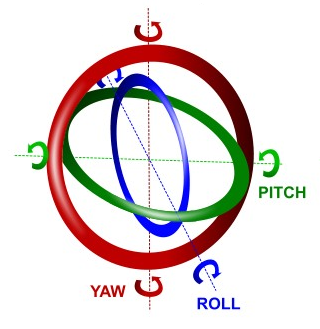
\includegraphics[width=0.42\textwidth]{estadodelarte/gimbal}
	\caption{Esquema estructura gimbal}
	\label{gimbal}
\end{figure}

Estas plataformas permiten que la aeronave gire entorno a su centro de gravedad, por lo que se reduce la influencia del peso de la aeronave en el control. Además es posible medir los ángulos de euler de la aeronave de forma directa empleando encoders en los ejes de rotación.

Hay empresas que están empezando a comercializar estas plataformas, tanto orientadas para la labor investigadora en el campo de los cuadricópteros , como para la labor docente que se puede llevar a cabo empleando estas plataformas con ánimo didáctico, para el aprendizaje de algoritmos de control. 

En cuanto a las  plataformas orientadas a la investigación, se encuentra la plataforma FFT gyro , desarrollada por Eureka Dynamics.

\begin{figure}[htb!]
	\centering
	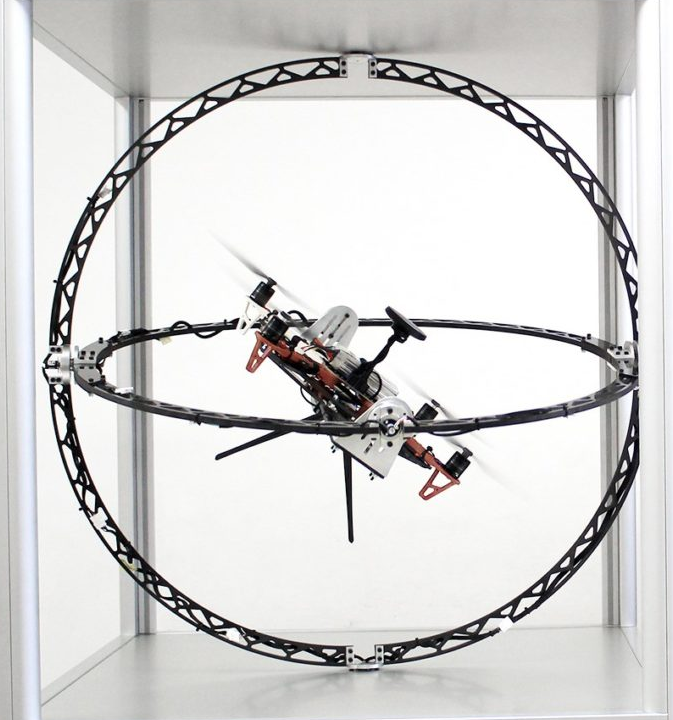
\includegraphics[width=0.6\textwidth]{estadodelarte/fft_gyro}
	\caption{Plataforma FFT Gyro de Eureka Dynamics}
	\label{giro_fft}
\end{figure}

Esta plataforma cuenta con encoders en cada eje de rotación para poder monitorizar el estado de la aeronave con gran precisión y esta construida en fibra de carbono para maximizar la rigidez de la estructura minimizando el peso.

\subsection{Plataformas con unión esférica}

Estas plataformas se unen a la aeronave a través de una unión esférica, la cual permite que el cuadricóptero pueda girar en tres ángulos, con algunas limitaciones. Por ejemplo, aunque en guiñada la aeronave pueda girar libremente, en alabeo y cabeceo este movimiento se ve restringido por las limitaciones mecánicas de la unión, véase \cref{union esferica}. Esto es una gran diferencia con respecto a las plataformas de tipo gimbal, en las que este suceso no ocurre, dado que en sus articulaciones no existen restricciones en los ángulos de giro.

A pesar de esto, estas plataformas condensan todos los giros en un único punto, por lo que el tamaño de la estructura requerida para anclar un cuadricóptero, es significativamente menor  que si se emplea una estructura de tipo gimbal.

\begin{figure}[htb!]
	\centering
	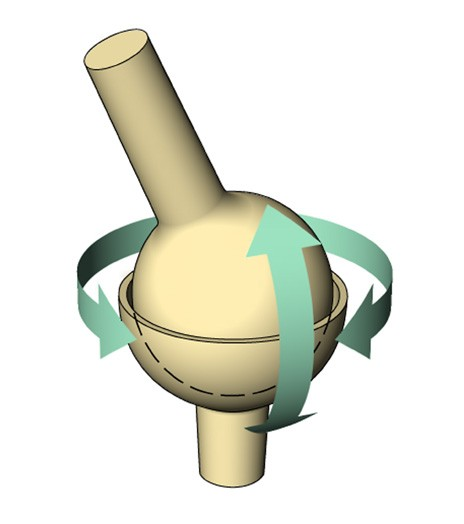
\includegraphics[width=0.4\textwidth]{estadodelarte/union_esferica}
	\caption{Esquema de una union esférica}
	\label{union esferica}
\end{figure}
\newpage
En cuanto a plataformas comerciales de esté tipo, cabe destacar las producidas por la empresa Quanser, la cuál ha desarrollado una plataforma con fines educativos, que emplea esta unión. Esta plataforma cuenta, al igual que la FFT Gyro con encoders, con la finalidad de conocer con precisión el estado de la aeronave.
   
\begin{figure}[htb!]
	\centering
	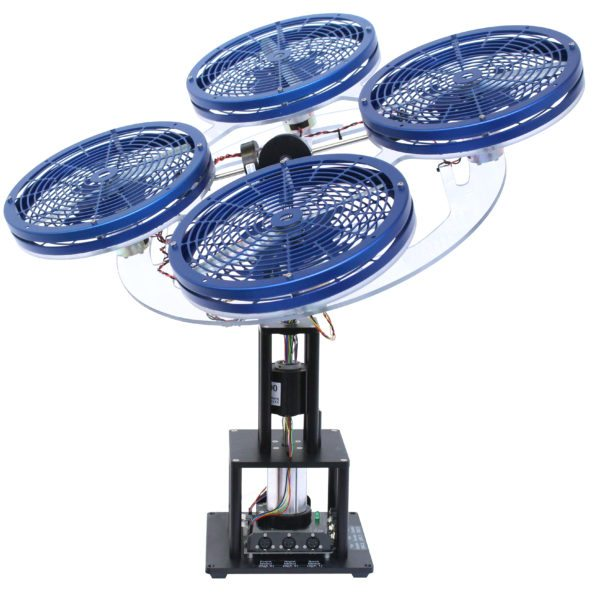
\includegraphics[width=0.5\textwidth]{estadodelarte/quanser}
	\caption{Plataforma 3 DOF Hover de la empresa Quanser}
	\label{union esferica}
\end{figure}

Entre las dos posibilidades, se ha optado por realizar una plataforma con una unión esférica debido a la mayor simplicidad y menor tamaño de este tipo de plataformas frente a su alternativa.
\section{Aprendizaje por refuerzo}
El aprendizaje por refuerzo o \textit{reinforcement learning} es una rama del aprendizaje automático en  la que un agente aprende a actuar a medida que va interactuando con su entorno. Es decir, el agente comienza realizando acciones aleatorias y va aprendiendo por ensayo-error. Para que el agente tenga noción de que acciones están ``bien'' y cuales no, el entorno proporciona una recompensa al agente en función de su comportamiento. Esta rama del aprendizaje automático se inspira en la psicología conductista.

Debido a esta capacidad de aprender de forma autónoma, sin necesidad de un conjunto previo de datos etiquetados, sino extrayendo información únicamente de su interacción con el entorno, estos algoritmos son muy empleados en el campo de la robótica para llevar a cabo tareas complicadas, tales como, aprender a andar o a manipular un cubo con destreza \cite{andrychowicz2018learning}.

Aunque existen una gran cantidad de ejemplos de uso de estas técnicas de aprendizaje en el ámbito de la robótica, en este trabajo se ha centrado en el empleo de estas técnicas al control de UAVs.

Los primeros experimentos en la utilización de algoritmos de control para UAVs, entrenados con aprendizaje con refuerzo, se llevaron a cabo con helicópteros. En 2004, HJ Kim et al. \cite{kim2004autonomous} emplearon algoritmos de \textit{reinforcement learning} para estabilizar (\textit{hover}) un helicóptero y conseguir realizar maniobras acrobáticas, para ello desarrollaron el algoritmo Pegasus \cite{ng2000pegasus}. Años después, en 2006 Andrew Y. et al \cite{ng2006autonomous} continuaron la investigación, en esta ocasión emplearon algoritmos que aprendían a realizar maniobras acrobáticas complejas, como mantener invertido al helicóptero. Para ello, realizaron un modelo estocástico no lineal de la dinámica del helicóptero, para, posteriormente, emplear ese modelo en simulación con el ánimo de generar un controlador capaz de estabilizar al helicóptero invertido.

En 2010 Travis Dierks et al. \cite{dierks2010output} desarrollaron un controlador no lineal, basado en redes neuronales, para estabilizar un cuadricóptero y seguir trayectorias. Para obtener un modelo completo de la aeronave, que fuera capaz también de tener en cuenta otros parámetros externos a la aeronave, como el coeficiente aerodinámico, el aprendizaje de la red neuronal se realizaba a tiempo real, mientras el cuadricóptero volaba. 

Unos años después, en 2017 Jemin Hwangbo et al. \cite{hwangbo2017control} desarrollaron un método para controlar un cuadricóptero con una red neuronal usando técnicas de \textit{reinforcement learning}. Desarrollaron un algoritmo, basado en la optimización determinista de la política y empleando descenso de gradientes natural para optimizar la misma. Consiguieron que el cuadricóptero fuera capaz de estabilizarse aún cuando partía de condiciones adversas, como ser lanzado casi boca abajo contra el suelo. Sin embargo, para conseguirlo, necesitaban frecuencias de actualización muy elevadas, del orden de los 100Khz, dos órdenes de magnitud mayor que un algoritmo típico.

 En 2018 William Koch et al. \cite{koch2019reinforcement} desarrollaron un entorno de simulación, GYMFC, para el desarrollo de nuevos algoritmos de control basados en redes neuronales. En su artículo compararon el rendimiento, en simulación, de distintos algoritmos de aprendizaje por refuerzo a la hora de cerrar el bucle de control en velocidad de un cuadricóptero. Posteriormente, a comienzos de 2019, desarrollaron Neuroflight \cite{koch2019neuroflight}, un \textit{firmware} para autopilotos \textit{open-source}. Este \textit{firmware}, a diferencia del de los autopilotos convencionales emplea bucles de control desarrollados con técnicas de aprendizaje por refuerzo, con los que consiguen controlar un cuadricóptero real. 

 